\PassOptionsToPackage{unicode}{hyperref}
\PassOptionsToPackage{hyphens}{url}
%\documentclass[9pt]{beamer} 
%\documentclass{beamer} 	%del imecc
\documentclass{beamer}
\usepackage{pgfpages}
\raggedbottom
\usepackage{beamerthemeshadow}
\usepackage{amsmath, amssymb, amsfonts, textcomp}
%=========================================================================================
\usepackage[brazilian]{babel}
% \usepackage[latin1]{inputenc}
\usepackage[utf8]{inputenc} % 
\usepackage{ragged2e}
\justifying
\setbeamertemplate{bibliography item}{[\theenumiv]}
\definecolor{airforceblue}{rgb}{0.36, 0.54, 0.66}
	%\definecolor{blue(ryb)}{rgb}{0.01, 0.28, 1.0}
\usetheme{Ilmenau}			% estilo y color de la presentacio
%\usetheme{JuanLesPins}		% estilo y color de la presentacio
\setbeamercolor{structure}{fg=airforceblue}
\mode<presentation>
\usepackage{times}
\usepackage[T1]{fontenc}	 %  
\usepackage{pgf, tikz}
\usetikzlibrary{arrows}
\usepackage{ stmaryrd }
%%
\usepackage{lmodern}
\usepackage{amssymb,amsmath}
\usepackage{ifxetex,ifluatex}
\ifnum 0\ifxetex 1\fi\ifluatex 1\fi=0 % if pdftex
  \usepackage[T1]{fontenc}
  \usepackage[utf8]{inputenc}
  \usepackage{textcomp} % provide euro and other symbols
\else % if luatex or xetex
  \usepackage{unicode-math}
  \defaultfontfeatures{Scale=MatchLowercase}
  \defaultfontfeatures[\rmfamily]{Ligatures=TeX,Scale=1}
\fi

\widowpenalties 1 10000
\raggedbottom

\providecommand{\tightlist}{%
  \setlength{\itemsep}{0pt}\setlength{\parskip}{0pt}}
\usepackage{color}
\usepackage{fancyvrb}
\newcommand{\VerbBar}{|}
\newcommand{\VERB}{\Verb[commandchars=\\\{\}]}
\DefineVerbatimEnvironment{Highlighting}{Verbatim}{commandchars=\\\{\}}
\usepackage{framed}
\definecolor{shadecolor}{RGB}{248,248,248}
\newenvironment{Shaded}{\begin{snugshade}}{\end{snugshade}}
\newcommand{\AlertTok}[1]{\textcolor[rgb]{0.94,0.16,0.16}{#1}}
\newcommand{\AnnotationTok}[1]{\textcolor[rgb]{0.56,0.35,0.01}{\textbf{\textit{#1}}}}
\newcommand{\AttributeTok}[1]{\textcolor[rgb]{0.77,0.63,0.00}{#1}}
\newcommand{\BaseNTok}[1]{\textcolor[rgb]{0.00,0.00,0.81}{#1}}
\newcommand{\BuiltInTok}[1]{#1}
\newcommand{\CharTok}[1]{\textcolor[rgb]{0.31,0.60,0.02}{#1}}
\newcommand{\CommentTok}[1]{\textcolor[rgb]{0.56,0.35,0.01}{\textit{#1}}}
\newcommand{\CommentVarTok}[1]{\textcolor[rgb]{0.56,0.35,0.01}{\textbf{\textit{#1}}}}
\newcommand{\ConstantTok}[1]{\textcolor[rgb]{0.00,0.00,0.00}{#1}}
\newcommand{\ControlFlowTok}[1]{\textcolor[rgb]{0.13,0.29,0.53}{\textbf{#1}}}
\newcommand{\DataTypeTok}[1]{\textcolor[rgb]{0.13,0.29,0.53}{#1}}
\newcommand{\DecValTok}[1]{\textcolor[rgb]{0.00,0.00,0.81}{#1}}
\newcommand{\DocumentationTok}[1]{\textcolor[rgb]{0.56,0.35,0.01}{\textbf{\textit{#1}}}}
\newcommand{\ErrorTok}[1]{\textcolor[rgb]{0.64,0.00,0.00}{\textbf{#1}}}
\newcommand{\ExtensionTok}[1]{#1}
\newcommand{\FloatTok}[1]{\textcolor[rgb]{0.00,0.00,0.81}{#1}}
\newcommand{\FunctionTok}[1]{\textcolor[rgb]{0.00,0.00,0.00}{#1}}
\newcommand{\ImportTok}[1]{#1}
\newcommand{\InformationTok}[1]{\textcolor[rgb]{0.56,0.35,0.01}{\textbf{\textit{#1}}}}
\newcommand{\KeywordTok}[1]{\textcolor[rgb]{0.13,0.29,0.53}{\textbf{#1}}}
\newcommand{\NormalTok}[1]{#1}
\newcommand{\OperatorTok}[1]{\textcolor[rgb]{0.81,0.36,0.00}{\textbf{#1}}}
\newcommand{\OtherTok}[1]{\textcolor[rgb]{0.56,0.35,0.01}{#1}}
\newcommand{\PreprocessorTok}[1]{\textcolor[rgb]{0.56,0.35,0.01}{\textit{#1}}}
\newcommand{\RegionMarkerTok}[1]{#1}
\newcommand{\SpecialCharTok}[1]{\textcolor[rgb]{0.00,0.00,0.00}{#1}}
\newcommand{\SpecialStringTok}[1]{\textcolor[rgb]{0.31,0.60,0.02}{#1}}
\newcommand{\StringTok}[1]{\textcolor[rgb]{0.31,0.60,0.02}{#1}}
\newcommand{\VariableTok}[1]{\textcolor[rgb]{0.00,0.00,0.00}{#1}}
\newcommand{\VerbatimStringTok}[1]{\textcolor[rgb]{0.31,0.60,0.02}{#1}}
\newcommand{\WarningTok}[1]{\textcolor[rgb]{0.56,0.35,0.01}{\textbf{\textit{#1}}}}
\usepackage{longtable,booktabs}
\usepackage{caption}
\usepackage{multicol}
%~~~~~~~~~~~~~~~~~~~~~~~~~~~
\usepackage{bbm}
\usepackage{eufrak}
\usepackage[mathscr]{euscript}
\usefonttheme{serif}
%~~~~~~~~~~~~~~~~~~~~~~~~~~~
% \pgfdeclareimage[height=1.0cm]{logo}{logounicamp}
\pgfdeclareimage[height=1.0cm]{encpos2020}{Figuras/encpos2020}
\logo{\pgfuseimage{encpos2020}}
% - - - - - - - - - - - - - - - - - - - - - - - - - - - - - - - - - - - - - - - - - - -
% figura 
\usepackage{subfig}
% \captionsetup[subfigure]{style=default, margin=0pt, parskip=0pt, hangindent=0pt, indention=0pt, singlelinecheck=true, labelformat=parens, labelsep=space}
% Caso queira guardar as figuras em uma pasta separada% - - - - - - - - - - - - - - - - - - - - 
% (descomente e) defina o caminho para o diretório:
%\graphicspath{{./figuras/}}

% Customizar as legendas de figuras e tabelas
\usepackage{caption}
\usepackage{empheq}

\newcommand{\vazio}{\emptyset}
\newcommand{\set}[1]{\left\{#1\right\}}

%%%%%%%%%%%%%%%%%%%%%%%%%%%%%%%%%%%%%%%%%%%%%%%%%%%%%%%%%
\usepackage{bm}
\newcommand{\lp}{\left(}% abrir par\^{e}nteses
\newcommand{\rp}{\right)}% fechar par\^{e}nteses
\newcommand{\qc}{\stackrel {{\rm q.c}}{\longrightarrow}}
\newcommand{\iid}{\stackrel {{\rm iid}}{\sim}}
\newcommand{\ind}{\stackrel {{\rm ind}}{\sim}}
\newcommand{\dd}{\stackrel {{\rm d}}{\longrightarrow}}
\newcommand{\sumi}{\sum^n_{i=1}}
\newcommand{\sumj}{\sum^g_{j=1}}
\newcommand{\sumas}{\sum^n_{i=1}}
\newcommand{\ii}{i=1,\ldots,n}
\newcommand{\ts}{t=1,\ldots,T}
\newcommand{\jj}{j=1,\ldots,n}
\newcommand{\by}{{\bf y}}
\newcommand{\yp}{\mathbf{y}}
\newcommand{\Y}{\mathbf{Y}}
%\newcommand{\vari}{\phi_b\textbf{u}_j\textbf{u}'_j+\mathbb{I}_{n_j}\phi_e}
\newcommand{\D}{\textrm{D}^{-1}(\bphi)}
\newcommand{\z}{\mathbf{Z}}
\newcommand{\Z}{\mathbf{Z}}
\newcommand{\zp}{\mathbf{z}}
\newcommand{\bA}{\mathbf{A}}
\newcommand{\A}{\textrm{A}}
\newcommand{\ap}{\mathbf{a}}
\newcommand{\X}{\mathbf{X}}
\newcommand{\R}{\mathbf{R}}
%\newcommand{\C}{\mathbf{C}}
\newcommand{\E}{\textrm{E}}
\newcommand{\up}{\mathbf{u}}
%\newcommand{\U}{\mathbf{U}}
\newcommand{\s}{\mathbf{s}}
\newcommand{\B}{\mathbf{B}}
\newcommand{\ST}{\textrm{ST}}
\newcommand{\SSL}{\textrm{SSL}}
\newcommand{\SCN}{\textrm{SCN}}
\newcommand{\SN}{\textrm{SN}}
\newcommand{\SNI}{\textrm{SNI}}
\newcommand{\NI}{\textrm{NI}}
\newcommand{\y}{\mathbf{y}}
\newcommand{\bF}{\mathbf{F}}
\newcommand{\bQ}{\mathbf{Q}}
\newcommand{\bC}{\mathbf{C}}
\newcommand{\bD}{\mathbf{D}}
\newcommand{\bc}{\mathbf{c}}
\newcommand{\bV}{\mathbf{V}}
\newcommand{\bv}{\mathbf{v}}
\newcommand{\bu}{\mathbf{u}}
\newcommand{\bx}{\mathbf{x}}
\newcommand{\xp}{\mathbf{x}}
\newcommand{\ba}{\mathbf{b}}
%-----------------------------------------------------------------
\newcommand{\balpha}{\mbox{${ \bm \alpha}$}}
\newcommand{\bmu}{\mbox{${ \bm \mu}$}}
\newcommand{\bphi}{\mbox{${ \bm \phi}$}}
\newcommand{\bPhi}{\mbox{${ \bm \Phi}$}}
\newcommand{\bnu}{\mbox{${ \bm \nu}$}}
\newcommand{\bSigma}{\mbox{${ \bm \Sigma}$}}
\newcommand{\bepsilon}{\mbox{${ \bm \epsilon}$}}
\newcommand{\bLambda}{\mbox{${ \bm \Lambda}$}}
\newcommand{\bbeta}{\mbox{${\bm \beta}$}}
\newcommand{\btheta}{\mbox{${ \bm \theta}$}}
\newcommand{\bTheta}{\mbox{${ \bm \Theta}$}}
\newcommand{\bxi}{\mbox{${ \bm \xi}$}}
\newcommand{\bvarphi}{\mbox{${ \bm \varphi}$}}
\newcommand{\bnabla}{\mbox{${ \bm \nabla}$}}
\newcommand{\bDelta}{\mbox{${ \bm \Delta}$}}
\newcommand{\bdelta}{\mbox{${ \bm \delta}$}}
\newcommand{\bPsi}{\mbox{${ \bm \Psi}$}}
\newcommand{\bpsi}{\mbox{${ \bm \psi}$}}
\newcommand{\btau}{\mbox{${ \bm \tau}$}}
\newcommand{\be}{\mathbf{b}}
\newcommand{\bpi}{\mbox{${ \bm \pi}$}}
\newcommand{\blambda}{\mbox{${ \bm \lambda}$}}
\newcommand{\bOmega}{\mbox{${ \bm \Omega}$}}
\newcommand{\bomega}{\mbox{${ \bm \omega}$}}
\newcommand{\bUpsilon}{\mbox{${ \bm \Upsilon}$}}
\newcommand{\bgamma}{\mbox{${ \bm \gamma}$}}
\newcommand{\bGamma}{\mbox{${ \bm \Gamma}$}}
\newcommand{\neta}{\mbox{${ \bm \eta}$}}
\newcommand{\bvar}{\mbox{${ \bm \varepsilon}$}}
\newcommand{\bS}{\mathbf{S}}
%
\newcommand{\bi}{\textbf{b}_i}
\newcommand{\bzeta}{\mbox{\boldmath $\zeta$}}
%
\newcommand{\sepvfill}{\setlength{\itemsep}{\fill}}

\begin{document}
%%TÍTULO-------------------------------------------
\author{Fernanda Lang Schumacher \\ \vspace{.2cm}\small joint work with Larissa A. Matos and Victor H. Lachos}
\title{Robust estimation in linear mixed models using the R package \it{skewlmm}}
\institute{Universidade Estadual de Campinas}
\titlegraphic{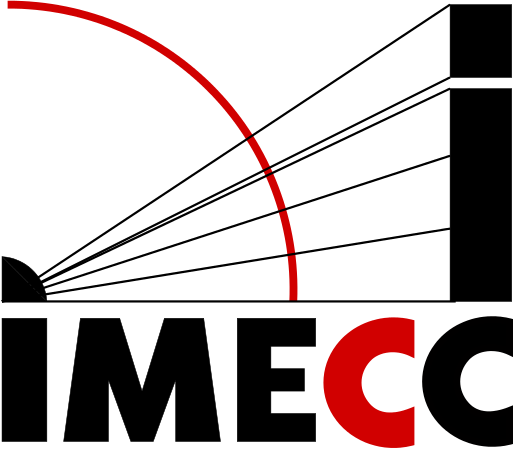
\includegraphics[width=1cm]{Figuras/imecc.png}~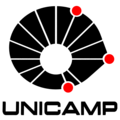
\includegraphics[width=1cm]{Figuras/logounicamp.png}}
\date{\today}

\frame{\maketitle}

% \AtBeginSection[]
% {  \begin{frame}<beamer>{Conteúdo}
%     \tableofcontents[currentsection]
%   \end{frame}}
%% - - - - - - - - - - - - - - - - - - - - - - - - - - - - - - - - - - - - - - - - - - -
% Conteudo do trabalho
\section{Introduction}

\begin{frame}
\frametitle{Introduction}
\begin{itemize}
\item Linear mixed models are frequently used to analyze repeated measures data.
\vfill\item Usual assumption: both random effect and error term follow normal
distributions. 
\vfill\item Some proposals have been made in the literature for relaxing the assumption of normality. \pause
\vfill\item Frequently, classes of LMMs consider that the error terms are conditionally independent. 
\vfill\item However, in longitudinal studies, repeated measures are collected over time and hence the error term tends to be serially correlated.
\end{itemize}
\end{frame}

\begin{frame}{Motivation: sleepstudy data}
\protect\hypertarget{motivation-sleepstudy-data}{}

\begin{itemize}
\tightlist
\item
  The average reaction time per day for subjects was evaluated by
  Gregory et al.~(2003) in a sleep deprivation study.
\vfill\item
  On day 0 the subjects had their normal amount of sleep and starting
  that night they were restricted to 3 hours of sleep per night for 9
  days, and the reaction time basead on a series of tests was measured
  on each day for each subject.
\vfill\item
  The data are available at the R package \emph{lme4}.
\end{itemize}

\end{frame}

\begin{frame}{Motivation: sleepstudy data}
\protect\hypertarget{motivation-sleepstudy-data-1}{}

\begin{center}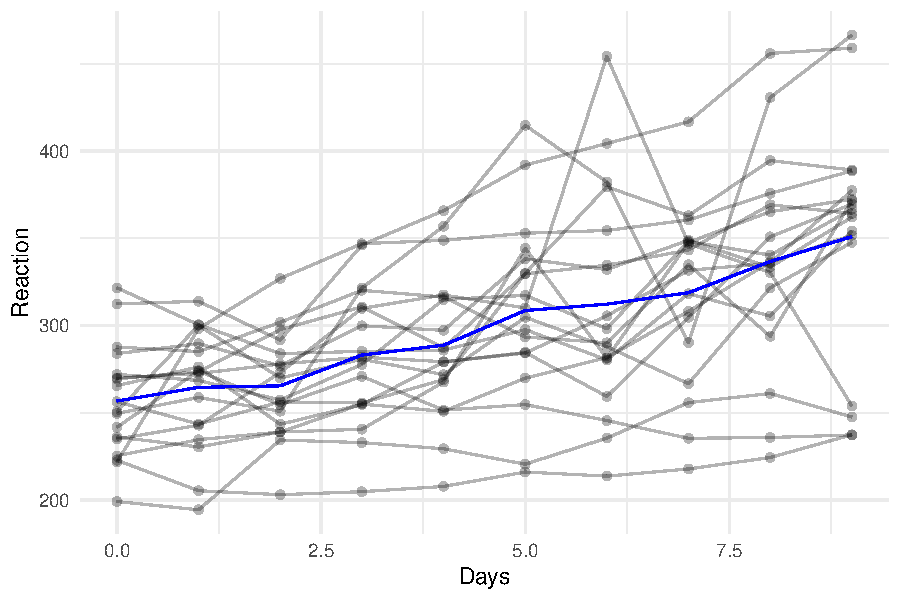
\includegraphics[width=0.85\linewidth]{codes_files/figure-beamer/data-1} \end{center}

\end{frame}

\begin{frame}[fragile]{Fitting a LMM to the sleepstudy dataset}
\protect\hypertarget{fitting-a-lmm-to-the-sleepstudy-dataset}{}

\begin{Shaded}
\begin{Highlighting}[]
\NormalTok{fitlme <-}\StringTok{ }\KeywordTok{lme}\NormalTok{(Reaction}\OperatorTok{~}\NormalTok{Days,}\DataTypeTok{data=}\NormalTok{sleepstudy,}
            \DataTypeTok{random=}\OperatorTok{~}\NormalTok{Days}\OperatorTok{|}\NormalTok{Subject)}
\end{Highlighting}
\end{Shaded}

%Plotting the random effects estimates obtained from the LMM:
\begin{center}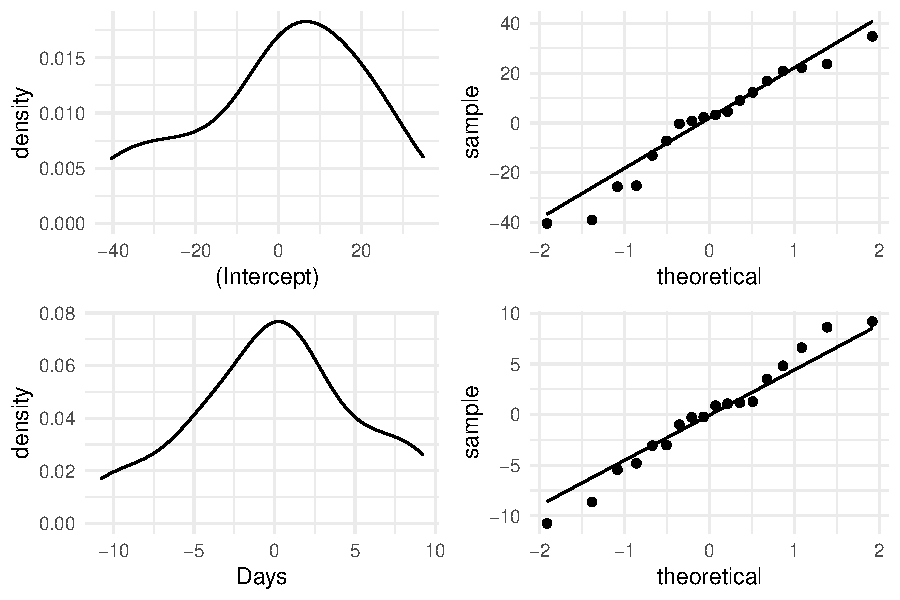
\includegraphics[width=0.7\linewidth]{codes_files/figure-beamer/fit1plot-1} \end{center}

\end{frame}

\section{Model formulation}
\begin{frame}\frametitle{Scale mixture of skew-normal (SMSN) distributions}
The $\textrm{SN}_p(\bmu,\bSigma,\mathbf{\blambda})$ distribution (Azzalini and Valle, 1996) can be defined from:
\begin{equation*}
    f(\mathbf{y})=2\phi_p(\mathbf{y};\bmu, \bSigma)
\Phi(A),\,\,\,\,\,\mathbf{y}\in \mathbb{R}^p,
\end{equation*}
where $A = \blambda^{\top}
\bSigma^{-1/2}\left(\mathbf{y}-\bmu\right)$.
\pause \vspace{.4cm}

The $\textrm{SMSN}_p(\bmu,\bSigma,\mathbf{\blambda};H)$ class of distributions can then be defined through the following pdf:
\begin{equation*}
f(\mathbf{y})=2\int_{0}^{\infty}\phi_p(\mathbf{y};\bmu,\kappa(u) \bSigma)\
\Phi(\kappa(u)^{-1/2} A)d H(u;\bnu),
\end{equation*}
$\mathbf{y}\in \mathbb{R}^p$, for some positive weight function $\kappa(u)$.
\end{frame}
%------------------------------------------------
\begin{frame}\frametitle{SMSN - special cases}
\begin{itemize}\setlength{\itemsep}{\fill}
    \item When $\blambda=0$, we get the $\textrm{SMN}_p(\bmu,\bSigma ;H)$;
    \item When  $\kappa(u)=u^{-1}$, we get the skew-normal/independent (SNI) class of distributions:
    \begin{itemize}\setlength{\itemsep}{.3cm}
        \item[-] By taking $U\sim \textrm{Gamma}(\nu/2,\nu/2)$, the $\ST_p(\bmu,\bSigma,\blambda,\nu)$ can be derived;
        \item[-] By taking $U\sim \textrm{Beta}(\nu,1)$, the $\SSL_p(\bmu,\bSigma,\blambda,\nu)$ can be derived;
        \item[-] By taking $U$ as a discrete random variable with probability function given by  $h(u|\bnu)=\nu_1 \mathbb{I}_{\{\nu_2\}}(u)+(1-\nu_1) \mathbb{I}_{\{1\}}(u)$, the $\SCN_p(\bmu,\bSigma,\blambda,\nu,\rho)$ can be derived, where $\nu_1,\nu_2\in (0,1)$.
    \end{itemize}
\end{itemize}
\end{frame}
%------------------------------------------------
\begin{frame}\frametitle{SMSN linear mixed model (SMSN-LMM)}
In general, a normal linear mixed effects model is defined as
\begin{equation}
\textbf{Y}_i=\textbf{X}_i\bbeta+\textbf{Z}_i\textbf{b}_i+\bepsilon_i,\,\,\,\,\ii\,,
\label{modeleq}
\end{equation}
where
\begin{itemize}
    \item $\textbf{X}_i$ of dimension $n_i\times l$ is the design matrix corresponding to the fixed effects, 
    \item $\bbeta$ of dimension $l\times 1$ is a vector of population-averaged regression coefficients called fixed effects, \item $\textbf{Z}_i$ of dimension $n_i\times q$  is the design matrix corresponding to the $q\times 1$ random effects vector $\textbf{b}_i$, and 
    \item $\bepsilon_i$ of dimension $n_i\times 1$ is the vector of random errors.
\end{itemize}
\end{frame}
%------------------------------------------------
\begin{frame}\frametitle{SMSN-LMM}
Usual assumptions:
\begin{itemize}
    \item $\textbf{b}_i\iid N_q(\mathbf{0},\textbf{D})$ $\perp$ $\bepsilon_i\ind N_{n_i}(\mathbf{0},\bSigma_i)$,
    \item The $q \times q$  random effects covariance matrix $\textbf{D}$ may be unstructured or structured,
    \item the $n_i \times n_i$ error covariance matrix $\bSigma_i$ is commonly written as $\sigma_e^2 \R_i$, where $\R_i$ can be a known matrix or a structured matrix depending on a vector of parameter, say $\bphi$.
\end{itemize}
\end{frame}
%------------------------------------------------
\begin{frame}\frametitle{SMSN-LMM}
Likewise, the SMSN-LMM can be defined by considering
\begin{equation}\label{modSnmis}
    \left( \begin{array}{c}
         \textbf{b}_i \\
         \bepsilon_i
    \end{array}\right) \ind \textrm{SMSN}_{q+n_i}
    \left( \left(\begin{array}{c}
         c\bDelta \\
         \mathbf{0}
    \end{array} \right), \left(\begin{array}{cc}
         \mathbf{D} & \mathbf{0} \\
         \mathbf{0} & \bSigma_i
    \end{array} \right), \left(\begin{array}{c}
         \blambda \\
         \mathbf{0}
    \end{array} \right); H \right),
\end{equation}
$\ii$, where 
\begin{itemize}
    \item $c= c(\bnu)=-\sqrt{\frac{2}{\pi}}k_1$, $k_1=\E\{U^{-1/2}\}$, $\bDelta = \textbf{D}^{1/2} \bdelta$, 
    \item  $\textbf{D} = \textbf{D}(\balpha)$ depends on unknown and reduced parameter vector $\balpha$, and
    \item $\bSigma_i = \sigma_e^2 \R_i$, with $\R_i = \R_i(\bphi)$, $\bphi=(\phi_1,\hdots,\phi_p)^\top$, being a structured matrix.
\end{itemize}
\end{frame}

%------------------------------------------------
\begin{frame}\frametitle{Within-subject dependence structures}
\begin{enumerate}
    \item Conditional independence (CI): $\textbf{R}_i = \mathbf{I}_{n_i}$.
    \item Autoregressive dependence of order $p$ (AR($p$)): \begin{equation*}
\mathbf{R}_{i}=\mathbf{R}_{i}(\bphi)=\frac{1}{1-\phi_1\rho_1-\ldots -\phi_p\rho_p}[\rho_{|r-s|}],
\end{equation*}
where $\rho_1,\hdots,\rho_p$ are the theoretical autocorrelations of the process and functions of $\bphi = (\phi_1,\ldots,\phi_p)^\top$, and they satisfy the Yule-Walker equations.
\item Damped exponential correlation (DEC):
\begin{equation*}
    \textbf{R}_i = \textbf{R}_i(\phi_1,\phi_2,\textbf{t}_i) = \left[ \phi_1^{|t_{ij}-t_{ik}|^{\phi_2}}\right], \,\,\,\, 0<\phi_1<1,\,\, \phi_2>0.
\end{equation*}
\end{enumerate}
\end{frame}
%------------------------------------------------
\begin{frame}\frametitle{Important remark}
The SMSN-LMM can be written hierarchically as follows:
\vspace{-.2cm}\begin{eqnarray*}
    \Y_i|\bi,U_i=u_i &\ind& \textrm{N}_{n_i}\left(\textbf{X}_i\bbeta+\textbf{Z}_i\textbf{b}_i,
    u_i^{-1}\sigma_e^2\textbf{R}_i\right),\\
    \bi|T_i=t_i,U_i=u_i &\ind& \textrm{N}_{q}\left(\bDelta t_i,
    u_i^{-1}\bGamma\right),\\
    T_i|U_i=u_i &\ind& \textrm{TN}\left(c,u_i^{-1}, (c,\infty)\right), \,\textrm{ and }\\
    U_i &\ind&  \textrm{H}(\cdot;\bnu), 
    \end{eqnarray*}

\vspace{-.2cm}which are all independent, and TN$(\mu,\tau,(a,b))$ denotes the univariate normal distribution (N$(\mu,\tau)$) truncated on the interval $(a,b)$.

This representation is useful for the implementation of an EM-type algorithm, for details see Schumacher et al. (2020).
\end{frame}
%------------------------------------------------

\begin{frame}{Tools for model evaluation}
\protect\hypertarget{tools-for-model-evaluation}{}
\begin{itemize}\sepvfill
    \item Likelihood ratio (LR) test;
    \item Mahalanobis distance (known distribution);
    \item Healy-type plot;
    \item Empirical autocorrelation function (ACF) for standardized marginal residuals, which at lag $l$ can be defined as
\vspace{-.2cm}\begin{equation*}
    \widehat{\rho}(l) = \frac{\sum_{i=1}^n \sum_{\{ (j,k) |t_k-t_j=l\}} r_{it_j} r_{it_k} / N(l)}{
    \sum_{i=1}^n \sum_{j=1}^{n_i} r_{it_j}^2/N(0) },
\end{equation*}

\vspace{-.4cm}
where $\textbf{r}_i = \widehat{\bUpsilon}_i^{-1/2}\left(\y_i - \textbf{X}_i\widehat{\bbeta} \right)$ is the standardized marginal residual vector for subject $i$, with $\bUpsilon_i=\text{Var}(\Y_i)$, and $N(\cdot)$ is the number of pairs used in the respective numerator summation.
\end{itemize}

\end{frame}

\section{The skewlmm package}
\begin{frame}[fragile]{The \texttt{R} package \emph{skewlmm}}
\protect\hypertarget{the-package}{}

\begin{itemize}\sepvfill
\item
  The package \emph{skewlmm} implemets an EM-type algorithm in
  \texttt{R} using S3 class, containing methods for estimating and
  predicting the SM(S)N-LMM.
\item
  It has an user-friendly interface with generic \texttt{R} functions
  \texttt{print}, \texttt{summary}, \texttt{plot}, \texttt{fitted},
  \texttt{residuals} and \texttt{predict} implemented.
\item
  The main functions in the package are \texttt{smsn.lmm()} and
  \texttt{smn.lmm()}, which fit a SMSN-LMM and a SMN-LMM, respectively.
\end{itemize}

\end{frame}

\begin{frame}[fragile]{The \texttt{R} package \emph{skewlmm}}
\protect\hypertarget{the-package-1}{}

The basic syntax of these functions is as follows:

\begin{Shaded}
\begin{Highlighting}[]
\KeywordTok{smsn.lmm}\NormalTok{(data, formFixed, groupVar, formRandom, }
\NormalTok{         depStruct, distr, ...)}
\KeywordTok{smn.lmm}\NormalTok{(data, formFixed, groupVar, formRandom, }
\NormalTok{        depStruct, distr, ...)}
\end{Highlighting}
\end{Shaded}

where

\begin{itemize}
\item
  \texttt{data}: A data frame containing all the variables to be used in
  the model.
\item
  \texttt{formFixed}: A two-sided linear formula object describing the
  fixed effects part of the model.
\item
  \texttt{groupVar}: A character containing the name of the variable
  which represents the subjects or groups in data.
\end{itemize}

\end{frame}

\begin{frame}[fragile]

\begin{itemize}
\item
  \texttt{formRandom}: A one-sided linear formula object describing the
  random effects part of the model.
\item
  \texttt{depStruct}: A character indicating which dependence structure
  should be used.
\item
  \texttt{distr}: A character indicating which distribution should be
  used.\pause
\end{itemize}

Some other useful arguments:

\begin{itemize}
\item
  \texttt{timeVar}: A character containing the name of the variable
  which represents the time in data.
\item
  \texttt{pAR}: The order of the autoregressive process that should be
  used (if depStruct=``ARp'').
\item
  \texttt{initialValues}: A named list containing initial parameter
  values.
\end{itemize}

\end{frame}

\begin{frame}[fragile]

The functions return an object of the class \texttt{SMSN} and
\texttt{SMN}, respectively, containing a list of elements, and the
following methods/ functions are available to these classes:

\begin{multicols}{2}
\begin{itemize}
\item
  \texttt{print}
\item
  \texttt{summary}
\item
  \texttt{fitted}
\item
  \texttt{plot}
\item
  \texttt{predict}
\item
  \texttt{residuals}
\item
  \texttt{ranef}
\item
  \texttt{acfresid}
\item
  \texttt{healy.plot}
\item
  \texttt{lr.test}
\item
  \texttt{mahalDist} 
\end{itemize}
\end{multicols}

\end{frame}
%%%%%%%%%%%%%%%%%%%%%%%%%%%%%%%%%%%%%%%%%%%%%%
\begin{frame}[fragile]{Example: sleepstudy data}
\protect\hypertarget{example-sleepstudy-data}{}

\scriptsize

\begin{Shaded}
\begin{Highlighting}[]
\CommentTok{#fitting a (CI)-SMN-LMM, default is distr='norm'}
\NormalTok{fit0<-}\KeywordTok{smn.lmm}\NormalTok{(}\DataTypeTok{data=}\NormalTok{sleepstudy,}\DataTypeTok{formFixed =}\NormalTok{ Reaction}\OperatorTok{~}\NormalTok{Days,}
              \DataTypeTok{formRandom =} \OperatorTok{~}\NormalTok{Days,}\DataTypeTok{groupVar =} \StringTok{"Subject"}\NormalTok{,}\DataTypeTok{quiet =}\NormalTok{ T)}
\end{Highlighting}
\end{Shaded}


\begin{Shaded}
\begin{Highlighting}[]
\CommentTok{#fitting a (CI)-SMSN-LMM, default is distr='sn'}
\NormalTok{fitskew0<-}\KeywordTok{smsn.lmm}\NormalTok{(}\DataTypeTok{data=}\NormalTok{sleepstudy,}\DataTypeTok{formFixed =}\NormalTok{ Reaction}\OperatorTok{~}\NormalTok{Days,}
              \DataTypeTok{formRandom =} \OperatorTok{~}\NormalTok{Days,}\DataTypeTok{groupVar =} \StringTok{"Subject"}\NormalTok{,}\DataTypeTok{quiet =}\NormalTok{ T)}
\end{Highlighting}
\end{Shaded}

\end{frame}

\begin{frame}[fragile]
\tiny

\begin{Shaded}
\begin{Highlighting}[]
\NormalTok{fit0}
\end{Highlighting}
\end{Shaded}

\begin{verbatim}
## Linear mixed models with distribution norm and dependency structure CI 
## Call:
## smn.lmm(data = sleepstudy, formFixed = Reaction ~ Days, groupVar = "Subject", 
##     formRandom = ~Days, quiet = T)
## 
## Fixed:Reaction ~ Days
## Random:~Days
##   Estimated variance (D):
##             (Intercept)     Days
## (Intercept)   560.68002 11.91827
## Days           11.91827 32.52525
## 
## Estimated parameters:
##      (Intercept)    Days   sigma2  Dsqrt1 Dsqrt2 Dsqrt3
##         251.4051 10.4673 655.4400 23.6752 0.4059 5.6886
## s.e.      7.2257  1.5541  31.3784 10.0856 1.7514 1.4270
## 
## Model selection criteria:
##   logLik     AIC      BIC
##  -875.97 1763.94 1783.098
## 
## Number of observations: 180 
## Number of groups: 18
\end{verbatim}

\end{frame}

\begin{frame}[fragile]

\tiny

\begin{Shaded}
\begin{Highlighting}[]
\NormalTok{fitskew0}
\end{Highlighting}
\end{Shaded}

\begin{verbatim}
## Linear mixed models with distribution sn and dependency structure CI 
## Call:
## smsn.lmm(data = sleepstudy, formFixed = Reaction ~ Days, groupVar = "Subject", 
##     formRandom = ~Days, quiet = T)
## 
## Fixed:Reaction ~ Days
## Random:~Days
##   Estimated variance (D):
##             (Intercept)     Days
## (Intercept)  1432.65701 35.22718
## Days           35.22718 33.76855
## 
## Estimated parameters:
##      (Intercept)    Days   sigma2  Dsqrt1 Dsqrt2 Dsqrt3 lambda1 lambda2
##         251.4073 10.4657 652.6598 37.8418 0.8080 5.7546 -4.2917 -0.2477
## s.e.     11.6328  2.1610  32.7878 28.9642 5.2063 1.6311      NA      NA
## 
## Model selection criteria:
##    logLik      AIC      BIC
##  -875.354 1766.709 1792.253
## 
## Number of observations: 180 
## Number of groups: 18
\end{verbatim}

\end{frame}

\begin{frame}[fragile]{Changing the distribution}
\protect\hypertarget{changing-the-distribution}{}

\scriptsize

\begin{Shaded}
\begin{Highlighting}[]
\NormalTok{fit1<-}\KeywordTok{smn.lmm}\NormalTok{(}\DataTypeTok{data=}\NormalTok{sleepstudy,}\DataTypeTok{formFixed =}\NormalTok{ Reaction}\OperatorTok{~}\NormalTok{Days,}\DataTypeTok{distr =} \StringTok{'t'}\NormalTok{,}
              \DataTypeTok{formRandom =} \OperatorTok{~}\NormalTok{Days,}\DataTypeTok{groupVar =} \StringTok{"Subject"}\NormalTok{,}\DataTypeTok{quiet =}\NormalTok{ T)}
\end{Highlighting}
\end{Shaded}

\begin{Shaded}
\begin{Highlighting}[]
\NormalTok{fitskew1<-}\KeywordTok{smsn.lmm}\NormalTok{(}\DataTypeTok{data=}\NormalTok{sleepstudy,}\DataTypeTok{formFixed =}\NormalTok{ Reaction}\OperatorTok{~}\NormalTok{Days,}\DataTypeTok{distr =} \StringTok{'st'}\NormalTok{,}
                  \DataTypeTok{formRandom =} \OperatorTok{~}\NormalTok{Days,}\DataTypeTok{groupVar =} \StringTok{"Subject"}\NormalTok{,}\DataTypeTok{quiet =}\NormalTok{ T)}
\end{Highlighting}
\end{Shaded}

\begin{Shaded}
\begin{Highlighting}[]
\NormalTok{fit2<-}\KeywordTok{smn.lmm}\NormalTok{(}\DataTypeTok{data=}\NormalTok{sleepstudy,}\DataTypeTok{formFixed =}\NormalTok{ Reaction}\OperatorTok{~}\NormalTok{Days,}\DataTypeTok{distr =} \StringTok{'sl'}\NormalTok{,}
              \DataTypeTok{formRandom =} \OperatorTok{~}\NormalTok{Days,}\DataTypeTok{groupVar =} \StringTok{"Subject"}\NormalTok{,}\DataTypeTok{quiet =}\NormalTok{ T)}
\end{Highlighting}
\end{Shaded}

\begin{Shaded}
\begin{Highlighting}[]
\NormalTok{fitskew2<-}\KeywordTok{smsn.lmm}\NormalTok{(}\DataTypeTok{data=}\NormalTok{sleepstudy,}\DataTypeTok{formFixed =}\NormalTok{ Reaction}\OperatorTok{~}\NormalTok{Days,}\DataTypeTok{distr =} \StringTok{'ssl'}\NormalTok{,}
                  \DataTypeTok{formRandom =} \OperatorTok{~}\NormalTok{Days,}\DataTypeTok{groupVar =} \StringTok{"Subject"}\NormalTok{,}\DataTypeTok{quiet =}\NormalTok{ T)}
\end{Highlighting}
\end{Shaded}

\begin{Shaded}
\begin{Highlighting}[]
\NormalTok{fit3<-}\KeywordTok{smn.lmm}\NormalTok{(}\DataTypeTok{data=}\NormalTok{sleepstudy,}\DataTypeTok{formFixed =}\NormalTok{ Reaction}\OperatorTok{~}\NormalTok{Days,}\DataTypeTok{distr =} \StringTok{'cn'}\NormalTok{,}
              \DataTypeTok{formRandom =} \OperatorTok{~}\NormalTok{Days,}\DataTypeTok{groupVar =} \StringTok{"Subject"}\NormalTok{,}\DataTypeTok{quiet =}\NormalTok{ T)}
\end{Highlighting}
\end{Shaded}

\begin{Shaded}
\begin{Highlighting}[]
\NormalTok{fitskew3<-}\KeywordTok{smsn.lmm}\NormalTok{(}\DataTypeTok{data=}\NormalTok{sleepstudy,}\DataTypeTok{formFixed =}\NormalTok{ Reaction}\OperatorTok{~}\NormalTok{Days,}\DataTypeTok{distr =} \StringTok{'scn'}\NormalTok{,}
                  \DataTypeTok{formRandom =} \OperatorTok{~}\NormalTok{Days,}\DataTypeTok{groupVar =} \StringTok{"Subject"}\NormalTok{,}\DataTypeTok{quiet =}\NormalTok{ T)}
\end{Highlighting}
\end{Shaded}

\end{frame}

\begin{frame}{Comparing the fitted models}
\protect\hypertarget{comparing-the-fitted-models}{}

\begin{longtable}[]{@{}crr@{}}
\toprule
distr & AIC & BIC\tabularnewline
\midrule
\endhead
norm & 1763.9 & 1783.1\tabularnewline
sn & 1766.7 & 1792.3\tabularnewline
t & 1737.5 & 1759.8\tabularnewline
st & 1739.8 & 1768.6\tabularnewline
sl & 1736.2 & \bf 1758.5\tabularnewline
ssl & 1738.4 & 1767.2\tabularnewline
cn & \bf 1733.7 & 1759.3\tabularnewline
scn & 1735.9 & 1767.8\tabularnewline
\bottomrule
\end{longtable}

\end{frame}

\begin{frame}[fragile]{Assessing the goodness of fit using a Healy-type
plot}
\protect\hypertarget{assessing-the-goodness-of-fit-using-a-healy-type-plot}{}

\scriptsize

\begin{Shaded}
\begin{Highlighting}[]
\KeywordTok{grid.arrange}\NormalTok{(}\KeywordTok{healy.plot}\NormalTok{(fit0),}\KeywordTok{healy.plot}\NormalTok{(fit1),}
             \KeywordTok{healy.plot}\NormalTok{(fit2),}\KeywordTok{healy.plot}\NormalTok{(fit3))}
\end{Highlighting}
\end{Shaded}

\begin{center}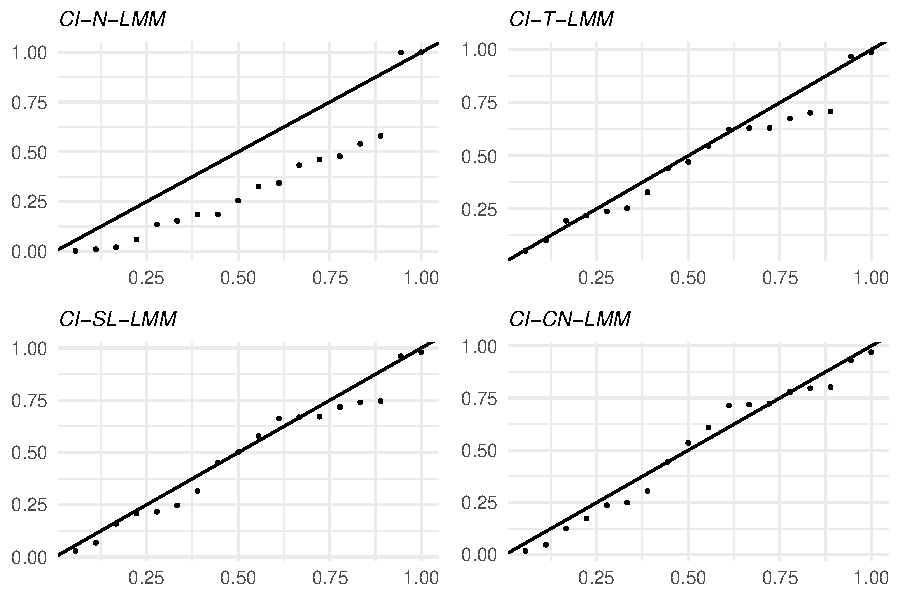
\includegraphics[width=0.75\linewidth]{codes_files/figure-beamer/healy1-1} \end{center}

\end{frame}

\begin{frame}[fragile]{LR test for \(H_0: \lambda=0\) in the CN-LMM}
\protect\hypertarget{lr-test-for-h_0-lambda0-in-the-cn-lmm}{}

\small

\begin{Shaded}
\begin{Highlighting}[]
\KeywordTok{lr.test}\NormalTok{(fitskew3,fit3)}
\end{Highlighting}
\end{Shaded}

\begin{verbatim}
## Model selection criteria:
##            logLik      AIC      BIC
## fitskew3 -857.926 1735.851 1767.781
## fit3     -858.861 1733.722 1759.266
## 
##     Likelihood-ratio Test
## 
## chi-square statistics =  1.871248 
## df =  2 
## p-value =  0.392341 
## 
## The null hypothesis that both models represent the 
## data equally well is not rejected at level  0.05
\end{verbatim}

\end{frame}

\begin{frame}[fragile]{Computing the ACF of the residuals from CN-LMM}
\protect\hypertarget{computing-the-acf-of-the-residuals-from-cn-lmm}{}

\begin{Shaded}
\begin{Highlighting}[]
\KeywordTok{acfresid}\NormalTok{(fit3)}
\end{Highlighting}
\end{Shaded}

\begin{verbatim}
##    lag         ACF n.used
## 1    0  1.00000000    180
## 2    1  0.19793878    162
## 3    2 -0.07329748    144
## 4    3 -0.21972223    126
## 5    4 -0.06519806    108
## 6    5 -0.13723727     90
## 7    6 -0.27485055     72
## 8    7 -0.08778128     54
## 9    8  0.19912222     36
## 10   9  0.58707921     18
\end{verbatim}

\end{frame}

\begin{frame}[fragile]{Plotting the ACF (CI-CN-LMM)}
\protect\hypertarget{plotting-the-acf-ci-cn-lmm}{}

\begin{Shaded}
\begin{Highlighting}[]
\KeywordTok{plot}\NormalTok{(}\KeywordTok{acfresid}\NormalTok{(fit3,}\DataTypeTok{calcCI =}\NormalTok{ T,}\DataTypeTok{maxLag =} \DecValTok{6}\NormalTok{))}
\end{Highlighting}
\end{Shaded}

\begin{center}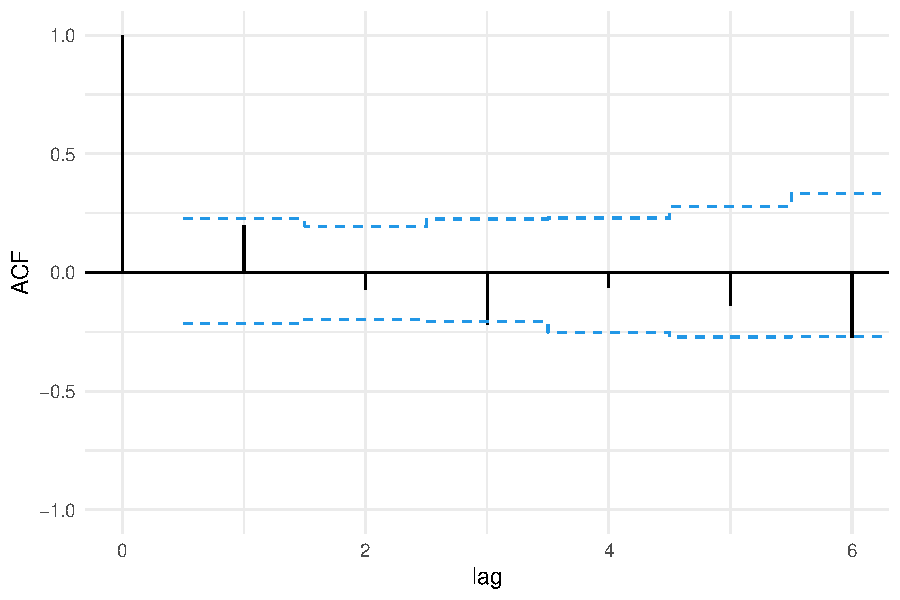
\includegraphics[width=0.7\linewidth]{codes_files/figure-beamer/fit6-1} \end{center}

\end{frame}

\begin{frame}[fragile]{Fitting an AR(p)-SMN-LMM}
\protect\hypertarget{fitting-an-arp-smn-lmm}{}

\scriptsize

\begin{Shaded}
\begin{Highlighting}[]
\CommentTok{#sl}
\NormalTok{fit2ar1<-}\KeywordTok{smn.lmm}\NormalTok{(}\DataTypeTok{data=}\NormalTok{sleepstudy,}\DataTypeTok{formFixed =}\NormalTok{ Reaction}\OperatorTok{~}\NormalTok{Days,}
                 \DataTypeTok{formRandom =} \OperatorTok{~}\NormalTok{Days,}\DataTypeTok{groupVar =} \StringTok{"Subject"}\NormalTok{,}
                 \DataTypeTok{distr=}\StringTok{"sl"}\NormalTok{,}\DataTypeTok{depStruct =} \StringTok{"ARp"}\NormalTok{,}\DataTypeTok{pAR=}\DecValTok{1}\NormalTok{,}\DataTypeTok{quiet=}\NormalTok{T)}
\end{Highlighting}
\end{Shaded}

\begin{Shaded}
\begin{Highlighting}[]
\NormalTok{fit2ar2<-}\KeywordTok{smn.lmm}\NormalTok{(}\DataTypeTok{data=}\NormalTok{sleepstudy,}\DataTypeTok{formFixed =}\NormalTok{ Reaction}\OperatorTok{~}\NormalTok{Days,}
                 \DataTypeTok{formRandom =} \OperatorTok{~}\NormalTok{Days,}\DataTypeTok{groupVar =} \StringTok{"Subject"}\NormalTok{,}
                 \DataTypeTok{distr=}\StringTok{"sl"}\NormalTok{,}\DataTypeTok{depStruct =} \StringTok{"ARp"}\NormalTok{,}\DataTypeTok{pAR=}\DecValTok{2}\NormalTok{,}\DataTypeTok{quiet=}\NormalTok{T)}
\end{Highlighting}
\end{Shaded}

\begin{Shaded}
\begin{Highlighting}[]
\CommentTok{#cn}
\NormalTok{fit3ar1<-}\KeywordTok{smn.lmm}\NormalTok{(}\DataTypeTok{data=}\NormalTok{sleepstudy,}\DataTypeTok{formFixed =}\NormalTok{ Reaction}\OperatorTok{~}\NormalTok{Days,}
                 \DataTypeTok{formRandom =} \OperatorTok{~}\NormalTok{Days,}\DataTypeTok{groupVar =} \StringTok{"Subject"}\NormalTok{,}
                 \DataTypeTok{distr=}\StringTok{"cn"}\NormalTok{,}\DataTypeTok{depStruct =} \StringTok{"ARp"}\NormalTok{,}\DataTypeTok{pAR=}\DecValTok{1}\NormalTok{,}\DataTypeTok{quiet=}\NormalTok{T)}
\end{Highlighting}
\end{Shaded}

\begin{Shaded}
\begin{Highlighting}[]
\NormalTok{fit3ar2<-}\KeywordTok{smn.lmm}\NormalTok{(}\DataTypeTok{data=}\NormalTok{sleepstudy,}\DataTypeTok{formFixed =}\NormalTok{ Reaction}\OperatorTok{~}\NormalTok{Days,}
                 \DataTypeTok{formRandom =} \OperatorTok{~}\NormalTok{Days,}\DataTypeTok{groupVar =} \StringTok{"Subject"}\NormalTok{,}
                 \DataTypeTok{distr=}\StringTok{"cn"}\NormalTok{,}\DataTypeTok{depStruct =} \StringTok{"ARp"}\NormalTok{,}\DataTypeTok{pAR=}\DecValTok{2}\NormalTok{,}\DataTypeTok{quiet=}\NormalTok{T)}
\end{Highlighting}
\end{Shaded}

\end{frame}

\begin{frame}[fragile]{Fitting a DEC-SMN-LMM}
\protect\hypertarget{fitting-a-dec-smn-lmm}{}

\scriptsize

\begin{Shaded}
\begin{Highlighting}[]
\CommentTok{#sl}
\NormalTok{fit2dec<-}\KeywordTok{smn.lmm}\NormalTok{(}\DataTypeTok{data=}\NormalTok{sleepstudy,}\DataTypeTok{formFixed =}\NormalTok{ Reaction}\OperatorTok{~}\NormalTok{Days,}
                 \DataTypeTok{formRandom =} \OperatorTok{~}\NormalTok{Days,}\DataTypeTok{groupVar =} \StringTok{"Subject"}\NormalTok{,}
                 \DataTypeTok{distr=}\StringTok{"sl"}\NormalTok{,}\DataTypeTok{depStruct =} \StringTok{"DEC"}\NormalTok{,}\DataTypeTok{quiet=}\NormalTok{T,}
                 \DataTypeTok{timeVar =} \StringTok{"Days"}\NormalTok{)}
\end{Highlighting}
\end{Shaded}

\begin{Shaded}
\begin{Highlighting}[]
\CommentTok{#cn}
\NormalTok{fit3dec<-}\KeywordTok{smn.lmm}\NormalTok{(}\DataTypeTok{data=}\NormalTok{sleepstudy,}\DataTypeTok{formFixed =}\NormalTok{ Reaction}\OperatorTok{~}\NormalTok{Days,}
                 \DataTypeTok{formRandom =} \OperatorTok{~}\NormalTok{Days,}\DataTypeTok{groupVar =} \StringTok{"Subject"}\NormalTok{,}
                 \DataTypeTok{distr=}\StringTok{"cn"}\NormalTok{,}\DataTypeTok{depStruct =} \StringTok{"DEC"}\NormalTok{,}\DataTypeTok{quiet=}\NormalTok{T,}
                 \DataTypeTok{timeVar =} \StringTok{"Days"}\NormalTok{)}
\end{Highlighting}
\end{Shaded}

\normalsize
Since the data are equally spaced and sorted by time, the use of
\texttt{timeVar} in here is optional (the function will use the position
if \texttt{timeVar} is not provided).

\end{frame}

\begin{frame}{Comparing the fitted models}
\protect\hypertarget{comparing-the-fitted-models-1}{}

\begin{longtable}[]{@{}llrr@{}}
\toprule
distr & depStruct & AIC & BIC\tabularnewline
\midrule
\endhead
sl & CI & 1736.2 & 1758.5\tabularnewline
sl & AR1 & 1716.9 & \bf 1742.5\tabularnewline
sl & AR2 & 1717.3 & 1746.0\tabularnewline
sl & DEC & 1718.2 & 1746.9\tabularnewline
cn & CI & 1733.7 & 1759.3\tabularnewline
cn & AR1 & 1715.5 & 1744.3\tabularnewline
cn & AR2 & \bf 1714.9 & 1746.9\tabularnewline
cn & DEC & 1716.3 & 1748.2\tabularnewline
\bottomrule
\end{longtable}

\end{frame}

\begin{frame}[fragile]{Healy plot for the AR(\(p\))-SMN-LMM}
\protect\hypertarget{healy-plot-for-the-arp-smn-lmm}{}

\scriptsize

\begin{Shaded}
\begin{Highlighting}[]
\KeywordTok{grid.arrange}\NormalTok{(}\KeywordTok{healy.plot}\NormalTok{(fit2ar1),}\KeywordTok{healy.plot}\NormalTok{(fit3ar1),}
            \KeywordTok{healy.plot}\NormalTok{(fit3ar2),}\DataTypeTok{ncol=}\DecValTok{2}\NormalTok{)}
\end{Highlighting}
\end{Shaded}

\begin{center}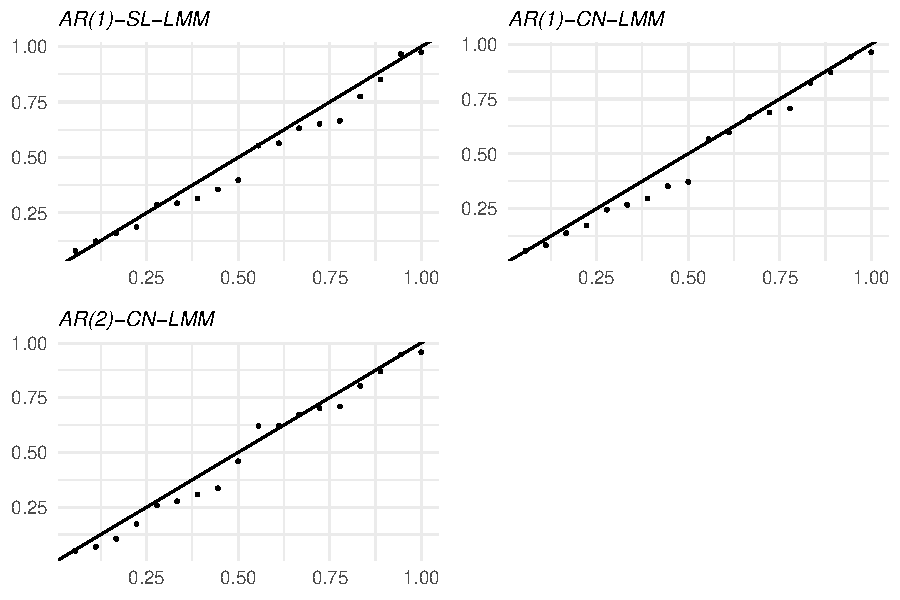
\includegraphics[width=0.75\linewidth]{codes_files/figure-beamer/healy2-1} \end{center}

\end{frame}

\begin{frame}[fragile]{LR test for \(H_0: \phi_2=0\) in the CN-LMM}
\protect\hypertarget{lr-test-for-h_0-phi_20-in-the-cn-lmm}{}

\scriptsize

\begin{Shaded}
\begin{Highlighting}[]
\KeywordTok{lr.test}\NormalTok{(fit3ar1,fit3ar2)}
\end{Highlighting}
\end{Shaded}

\begin{verbatim}
## 
## Model selection criteria:
##           logLik      AIC      BIC
## fit3ar1 -848.760 1715.520 1744.257
## fit3ar2 -847.463 1714.925 1746.855
## 
##     Likelihood-ratio Test
## 
## chi-square statistics =  2.594949 
## df =  1 
## p-value =  0.1072049 
## 
## The null hypothesis that both models represent the 
## data equally well is not rejected at level  0.05
\end{verbatim}

\end{frame}

\begin{frame}[fragile]{ACF plot for AR(1)-SMN-LMM}
\protect\hypertarget{acf-plot-for-ar1-smn-lmm}{}

\scriptsize

\begin{Shaded}
\begin{Highlighting}[]
\KeywordTok{grid.arrange}\NormalTok{(}\KeywordTok{plot}\NormalTok{(}\KeywordTok{acfresid}\NormalTok{(fit2ar1,}\DataTypeTok{calcCI =}\NormalTok{ T,}\DataTypeTok{maxLag =} \DecValTok{6}\NormalTok{))}\OperatorTok{+}
\StringTok{               }\KeywordTok{ggtitle}\NormalTok{(}\StringTok{"AR(1)-SL-LMM"}\NormalTok{),}
             \KeywordTok{plot}\NormalTok{(}\KeywordTok{acfresid}\NormalTok{(fit3ar1,}\DataTypeTok{calcCI =}\NormalTok{ T,}\DataTypeTok{maxLag =} \DecValTok{6}\NormalTok{))}\OperatorTok{+}
\StringTok{               }\KeywordTok{ggtitle}\NormalTok{(}\StringTok{"AR(1)-CN-LMM"}\NormalTok{), }\DataTypeTok{ncol=}\DecValTok{2}\NormalTok{)}
\end{Highlighting}
\end{Shaded}

\begin{center}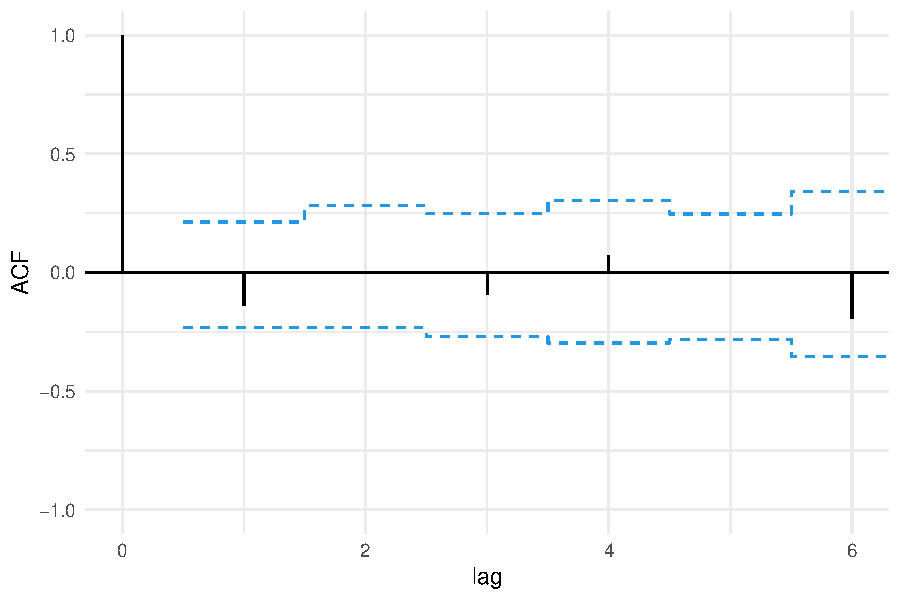
\includegraphics[width=0.8\linewidth]{codes_files/figure-beamer/acf1-1} \end{center}

\end{frame}

% \begin{frame}[fragile]{Fitted models}
% \protect\hypertarget{fitted-models}{}

% \scriptsize

% \begin{Shaded}
% \begin{Highlighting}[]
% \CommentTok{#sl}
% \KeywordTok{cbind}\NormalTok{(fit2ar1}\OperatorTok{$}\NormalTok{theta,fit2ar1}\OperatorTok{$}\NormalTok{std.error) }\OperatorTok\StringTok{ }
% \StringTok{  }\NormalTok{knitr}\OperatorTok{::}\KeywordTok{kable}\NormalTok{(}\DataTypeTok{digits =} \DecValTok{2}\NormalTok{,}\DataTypeTok{col.names =} \KeywordTok{c}\NormalTok{(}\StringTok{'estimate'}\NormalTok{,}\StringTok{'std.error'}\NormalTok{))}
% \end{Highlighting}
% \end{Shaded}

% \begin{longtable}[]{@{}lrr@{}}
% \toprule
% & estimate & std.error\tabularnewline
% \midrule
% \endhead
% (Intercept) & 251.55 & 7.56\tabularnewline
% Days & 9.81 & 1.66\tabularnewline
% sigma2 & 266.24 & 63.43\tabularnewline
% phiAR1 & 0.57 & 0.14\tabularnewline
% Dsqrt1 & 14.21 & 10.15\tabularnewline
% Dsqrt2 & 2.58 & 4.16\tabularnewline
% Dsqrt3 & 2.17 & 6.45\tabularnewline
% nu1 & 1.52 & NA\tabularnewline
% \bottomrule
% \end{longtable}

% \end{frame}

% \begin{frame}[fragile]

% \scriptsize

% \begin{Shaded}
% \begin{Highlighting}[]
% \CommentTok{#cn}
% \KeywordTok{cbind}\NormalTok{(fit3ar1}\OperatorTok{$}\NormalTok{theta,fit3ar1}\OperatorTok{$}\NormalTok{std.error) }\OperatorTok\StringTok{ }
% \StringTok{  }\NormalTok{knitr}\OperatorTok{::}\KeywordTok{kable}\NormalTok{(}\DataTypeTok{digits =} \DecValTok{2}\NormalTok{,}\DataTypeTok{col.names =} \KeywordTok{c}\NormalTok{(}\StringTok{'estimate'}\NormalTok{,}\StringTok{'std.error'}\NormalTok{))}
% \end{Highlighting}
% \end{Shaded}

% \begin{longtable}[]{@{}lrr@{}}
% \toprule
% & estimate & std.error\tabularnewline
% \midrule
% \endhead
% (Intercept) & 252.55 & 7.02\tabularnewline
% Days & 9.99 & 1.57\tabularnewline
% sigma2 & 417.84 & 78.77\tabularnewline
% phiAR1 & 0.56 & 0.14\tabularnewline
% Dsqrt1 & 16.90 & 11.82\tabularnewline
% Dsqrt2 & 2.82 & 4.76\tabularnewline
% Dsqrt3 & 2.89 & 6.31\tabularnewline
% nu1 & 0.12 & NA\tabularnewline
% nu2 & 0.16 & NA\tabularnewline
% \bottomrule
% \end{longtable}

% \end{frame}

\begin{frame}[fragile]{Fitted models}
\protect\hypertarget{fitted-models}{}

\scriptsize

\begin{Shaded}
\begin{Highlighting}[]
\KeywordTok{cbind}\NormalTok{(}\KeywordTok{c}\NormalTok{(fit2ar1}\OperatorTok{$}\NormalTok{theta,}\OtherTok{NA}\NormalTok{),}\KeywordTok{c}\NormalTok{(fit2ar1}\OperatorTok{$}\NormalTok{std.error,}\OtherTok{NA}\NormalTok{),}
\NormalTok{      fit3ar1}\OperatorTok{$}\NormalTok{theta,fit3ar1}\OperatorTok{$}\NormalTok{std.error) }
\end{Highlighting}
\end{Shaded}

\begin{longtable}[]{@{}lrrrr@{}}
\toprule
& \multicolumn{2}{c}{{SL}} &\multicolumn{2}{c}{{CN}}\tabularnewline
& estimate & std.error & estimate & std.error\tabularnewline
\midrule
\endhead
(Intercept) & 251.55 & 7.56 & 252.55 & 7.02\tabularnewline
Days & 9.81 & 1.66 & 9.99 & 1.57\tabularnewline
sigma2 & 266.24 & 63.43 & 417.84 & 78.77\tabularnewline
phiAR1 & 0.57 & 0.14 & 0.56 & 0.14\tabularnewline
Dsqrt1 & 14.21 & 10.15 & 16.90 & 11.82\tabularnewline
Dsqrt2 & 2.58 & 4.16 & 2.82 & 4.76\tabularnewline
Dsqrt3 & 2.17 & 6.45 & 2.89 & 6.31\tabularnewline
nu1 & 1.52 & NA & 0.12 & NA\tabularnewline
nu2& NA & NA & 0.16 & NA\tabularnewline
\bottomrule
\end{longtable}

\end{frame}


\begin{frame}[fragile]{Mahalanobis distance for AR(1)-SMN-LMM}
\protect\hypertarget{mahalanobis-distance-for-ar1-smn-lmm}{}

\scriptsize

\begin{Shaded}
\begin{Highlighting}[]
\KeywordTok{grid.arrange}\NormalTok{(}\KeywordTok{plot}\NormalTok{(}\KeywordTok{mahalDist}\NormalTok{(fit2ar1),}\DataTypeTok{fitobject =}\NormalTok{ fit2ar1,}\DataTypeTok{nlabels =} \DecValTok{0}\NormalTok{)}\OperatorTok{+}
\StringTok{               }\KeywordTok{ggtitle}\NormalTok{(}\StringTok{'AR(1)-SL-LMM'}\NormalTok{),}
             \KeywordTok{plot}\NormalTok{(}\KeywordTok{mahalDist}\NormalTok{(fit3ar1),}\DataTypeTok{fitobject =}\NormalTok{ fit3ar1,}\DataTypeTok{nlabels =} \DecValTok{0}\NormalTok{)}\OperatorTok{+}
\StringTok{               }\KeywordTok{ggtitle}\NormalTok{(}\StringTok{'AR(1)-CN-LMM'}\NormalTok{),} \DataTypeTok{ncol=}\DecValTok{2}\NormalTok{)}
\end{Highlighting}
\end{Shaded}

\begin{center}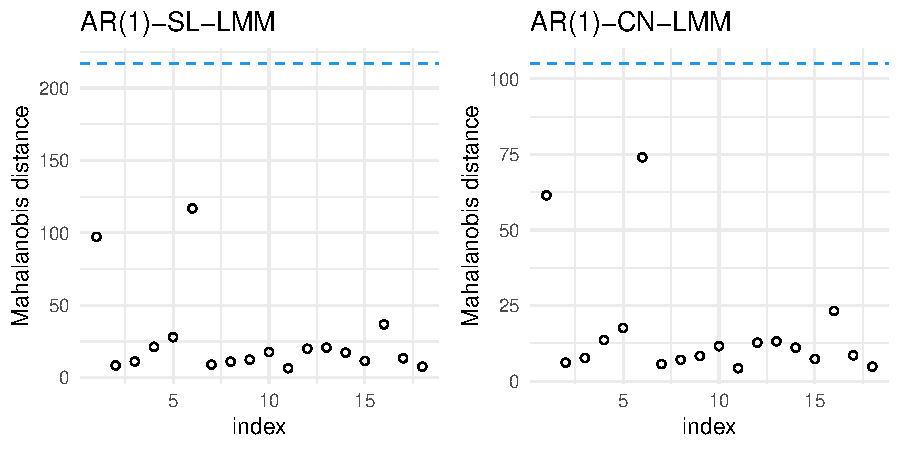
\includegraphics[width=0.8\linewidth]{codes_files/figure-beamer/mahal1-1} \end{center}

\end{frame}

\begin{frame}[fragile]{Mahalanobis distance versus \(\hat{u}\) for
AR(1)-SMN-LMM}
\protect\hypertarget{mahalanobis-distance-versus-hatu-for-ar1-smn-lmm}{}

\scriptsize

\begin{Shaded}
\begin{Highlighting}[]
\KeywordTok{grid.arrange}\NormalTok{(}\KeywordTok{qplot}\NormalTok{(}\KeywordTok{mahalDist}\NormalTok{(fit2ar1),fit2ar1}\OperatorTok{$}\NormalTok{uhat)}\OperatorTok{+}\KeywordTok{theme_minimal}\NormalTok{()}\OperatorTok{+}
\StringTok{               }\KeywordTok{ylab}\NormalTok{(}\StringTok{"uhat"}\NormalTok{)}\OperatorTok{+}\KeywordTok{xlab}\NormalTok{(}\StringTok{"Mahalanobis distance"}\NormalTok{)}\OperatorTok{+}
\StringTok{               }\KeywordTok{ggtitle}\NormalTok{(}\StringTok{'AR(1)-SL-LMM'}\NormalTok{),}
             \KeywordTok{qplot}\NormalTok{(}\KeywordTok{mahalDist}\NormalTok{(fit3ar1),fit3ar1}\OperatorTok{$}\NormalTok{uhat)}\OperatorTok{+}\KeywordTok{theme_minimal}\NormalTok{()}\OperatorTok{+}
\StringTok{               }\KeywordTok{ylab}\NormalTok{(}\StringTok{"uhat"}\NormalTok{)}\OperatorTok{+}\KeywordTok{xlab}\NormalTok{(}\StringTok{"Mahalanobis distance"}\NormalTok{)}\OperatorTok{+}
\StringTok{               }\KeywordTok{ggtitle}\NormalTok{(}\StringTok{'AR(1)-CN-LMM'}\NormalTok{),} \DataTypeTok{ncol=}\DecValTok{2}\NormalTok{)}
\end{Highlighting}
\end{Shaded}

\begin{center}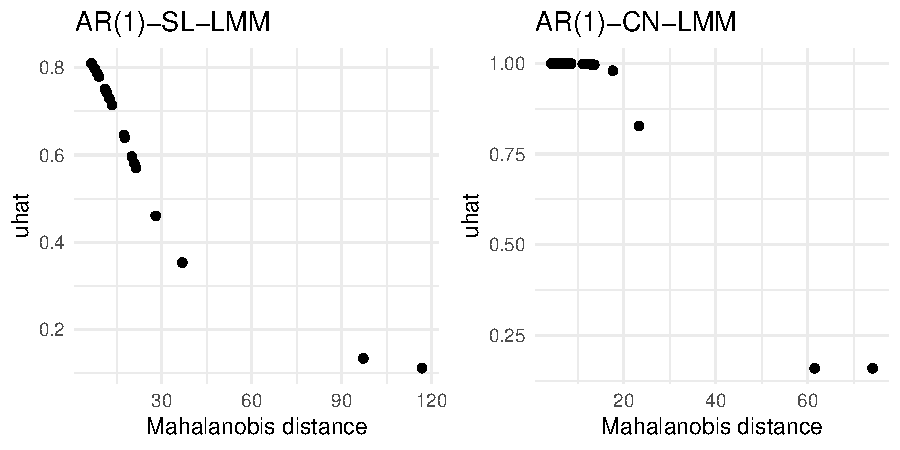
\includegraphics[width=0.8\linewidth]{codes_files/figure-beamer/mahal2-1} \end{center}

\end{frame}

\begin{frame}[fragile]{Plotting fitted models}
\protect\hypertarget{plot-fitted-models}{}

\scriptsize

\begin{Shaded}
\begin{Highlighting}[]
\KeywordTok{grid.arrange}\NormalTok{(}\KeywordTok{plot}\NormalTok{(fit2ar1,}\DataTypeTok{type =} \StringTok{"normalized"}\NormalTok{)}\OperatorTok{+}\KeywordTok{ggtitle}\NormalTok{(}\StringTok{'AR(1)-SL-LMM'}\NormalTok{),}
             \KeywordTok{plot}\NormalTok{(fit3ar1,}\DataTypeTok{type =} \StringTok{"normalized"}\NormalTok{)}\OperatorTok{+}\KeywordTok{ggtitle}\NormalTok{(}\StringTok{'AR(1)-CN-LMM'}\NormalTok{),}
             \DataTypeTok{ncol=}\DecValTok{2}\NormalTok{)}
\end{Highlighting}
\end{Shaded}

\begin{center}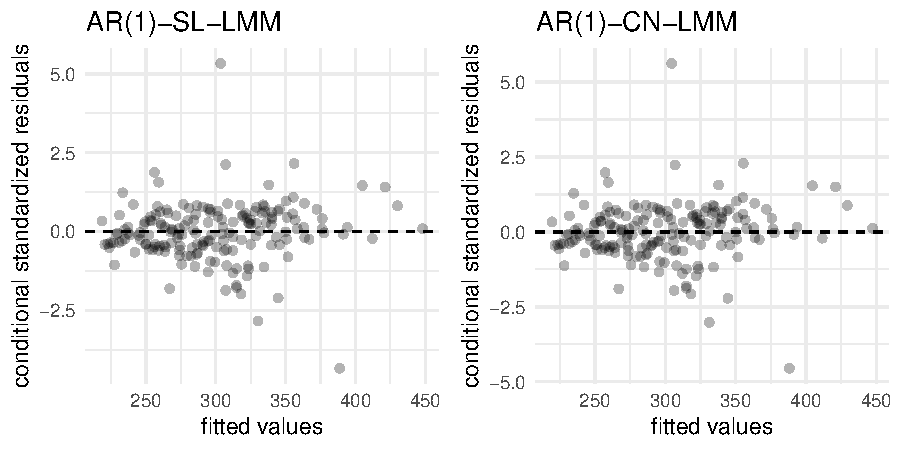
\includegraphics[width=0.85\linewidth]{codes_files/figure-beamer/extra1-1} \end{center}

\end{frame}

\begin{frame}[fragile]{Prediction of future measurements}
\protect\hypertarget{prediction-of-future-measurements}{}

\scriptsize

\begin{Shaded}
\begin{Highlighting}[]
\KeywordTok{tail}\NormalTok{(sleepstudy,}\DataTypeTok{n=}\DecValTok{3}\NormalTok{)}
\end{Highlighting}
\end{Shaded}

\begin{verbatim}
##     Reaction Days Subject
## 178 343.2199    7     372
## 179 369.1417    8     372
## 180 364.1236    9     372
\end{verbatim}

\begin{Shaded}
\begin{Highlighting}[]
\NormalTok{predData <-}\StringTok{ }\KeywordTok{data.frame}\NormalTok{(}\DataTypeTok{Reaction=}\OtherTok{NA}\NormalTok{,}\DataTypeTok{Days=}\DecValTok{10}\OperatorTok{:}\DecValTok{11}\NormalTok{,}\DataTypeTok{Subject=}\StringTok{"372"}\NormalTok{)}
\KeywordTok{predict}\NormalTok{(fit2ar1,}\DataTypeTok{newData =}\NormalTok{ predData)}
\end{Highlighting}
\end{Shaded}

\begin{verbatim}
##   groupVar Days    ypred
## 1      372   10 377.0998
## 2      372   11 389.5745
\end{verbatim}

\begin{Shaded}
\begin{Highlighting}[]
\KeywordTok{predict}\NormalTok{(fit3ar1,}\DataTypeTok{newData =}\NormalTok{ predData)}
\end{Highlighting}
\end{Shaded}

\begin{verbatim}
##   groupVar Days    ypred
## 1      372   10 377.1056
## 2      372   11 389.5576
\end{verbatim}

\end{frame}

\section{Concluding remarks}
\begin{frame}{Concluding remarks}
    Some additional features are currently under development:
    \begin{itemize}
        \item Estimation of some important special cases, such as when $\bD$ is diagonal or in blocks; 
        \item Use of parallel optimization to improve performance;
        \item Use of a method for acceleration of the convergence rate of the EM-type algorithm used in the estimation procedure. 
    \end{itemize}
\end{frame}

\begin{frame}{Main references}
\protect\hypertarget{references}{}
\vspace{-.2cm}
\tiny{
\begin{thebibliography}{99} % Beamer does not support BibTeX so references must be inserted manually as below
\bibitem{azzalini} Azzalini, A. \& A. D. Valle (1996).
\newblock The multivariate skew-normal distribution.
\newblock Biometrika 83(4), 715–726.

\bibitem{belenky} Belenky, G., Wesensten, N. J., Thorne, D. R., Thomas, M, L., Sing, H. C., Redmond, D. P., Russo, M. B. \& Balkin, T. J. (2003).
\newblock Patterns of performance degradation and restoration during sleep restriction and subsequent recovery: a sleep
  dose-response study. 
\newblock Journal of Sleep Research 12, 1--12.

\bibitem{box} Box, G. E., G. M. Jenkins, G. C. Reinsel \& G. M. Ljung (2015).
\newblock Time series analysis: forecasting and control.
\newblock John Wiley \& Sons.

\bibitem{dempster} Dempster, A., Laird, N. \& Rubin, D. (1977).
\newblock Maximum likelihood from incomplete data via the EM algorithm.
\newblock Journal of the Royal Statistical Society, Series B 39, 1–38.

\bibitem{lachos} Lachos, V. H., P. Ghosh \& R. B. Arellano-Valle (2010).
\newblock Likelihood based inference for skew–normal independent linear mixed models.
\newblock Statistica Sinica 20, 303–322.

\bibitem{munoz} Muñoz, A., V. Carey, J. P. Schouten, M. Segal \& B. Rosner (1992).
\newblock A parametric family of correlation structures for the analysis of longitudinal data.
\newblock Biometrics 48, 733–742.

\bibitem{schumacher} Schumacher, F. L., Matos, L. A., \& Lachos, V. H. (2020).
\newblock Scale mixture of skew-normal linear mixed models with within-subject serial dependence. 
\newblock arXiv preprint arXiv:2002.01040.

\end{thebibliography}
}
\end{frame}

\begin{frame}
%\vspace{-.5cm}
\begin{columns}
\column{.45\textwidth}
\begin{tabular}{cc}
         \large Preprint&  \large GitHub \\
         \href{https://arxiv.org/abs/2002.01040}{
\includegraphics[ height=2.2cm, keepaspectratio=true]{Figuras/paper-arxiv.png}}
         & \href{https://github.com/fernandalschumacher}{
\includegraphics[ height=2.2cm, keepaspectratio=true]{Figuras/github.png}}
\end{tabular}
\column{.49\textwidth}
\vspace{-.4cm}\center{\Large Acknowledgments} 
\\%
\includegraphics[ height=1.7cm, keepaspectratio=true]{imecc} \hspace{.5cm}

\includegraphics[ height=2.2cm, keepaspectratio=true]{Figuras/cnpq_capes.jpg}
\end{columns}

\vfill

\fboxsep=0pt
\noindent%
\begin{minipage}[t]{0.38\linewidth}
\begin{flushright} 
\vspace{.01cm}

\includegraphics[ height=1cm, keepaspectratio=true]{Figuras/contact.jpg}
\end{flushright}
\end{minipage}%
\hfill%
\begin{minipage}[t]{0.6\linewidth}
\begin{flushright} 
%\color{paynesgrey}
Fernanda Lang Schumacher\\
PhD student, IMECC -- UNICAMP\\
\color{black}
\nolinkurl{fernandalschumacher@gmail.com}
%\url{https://www.linkedin.com/in/fernanda-lang-schumacher-18123775}
\end{flushright}
\end{minipage}
%\center{\huge Thank you!}
\end{frame}


% - - - - - - - - - - - - - - - - - - - - - - - - - - - - - - - - - - - - - - - - - - - - - - - - - - - - - - - -
%\frame{ \frametitle{Principais Refer\^encias }

%\begin{enumerate}
%  \item
%  \item 
%\end{enumerate}
%}
%\emd{frame}
\end{document}

